\chapter{Datasets}\label{chapter:Datasets}

\begin{figure}[!ht]
	\centering
	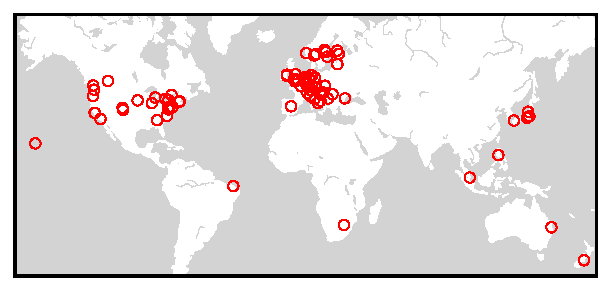
\includegraphics[keepaspectratio, height = 5cm, width=15cm]{figures/probes-geo-distribution.pdf}
	\caption[Probes Geographical Distribution]{Geographical Distribution of 100 dual-stacked SamKnows Probes. The probes takes hourly measurements of IPv4 and IPv6 towards Netflix CDN. The metadata for each probe is available online: https://goo.gl/NN81ij.}
	\label{fig:PROBES GEO DISTRIBUTION}
\end{figure}

\section{Methodology}
In this section, we will summarize the methodology of collecting the Netflix dataset. 
The data collection is not a contribution of this thesis, we will be just using the dataset to perform our analysis. 
We will explain the data collection technique in this section and will explain the dataset metrics and aggregation strategies in more detail in the next section. 

\begin{figure}[!ht]
	\centering
	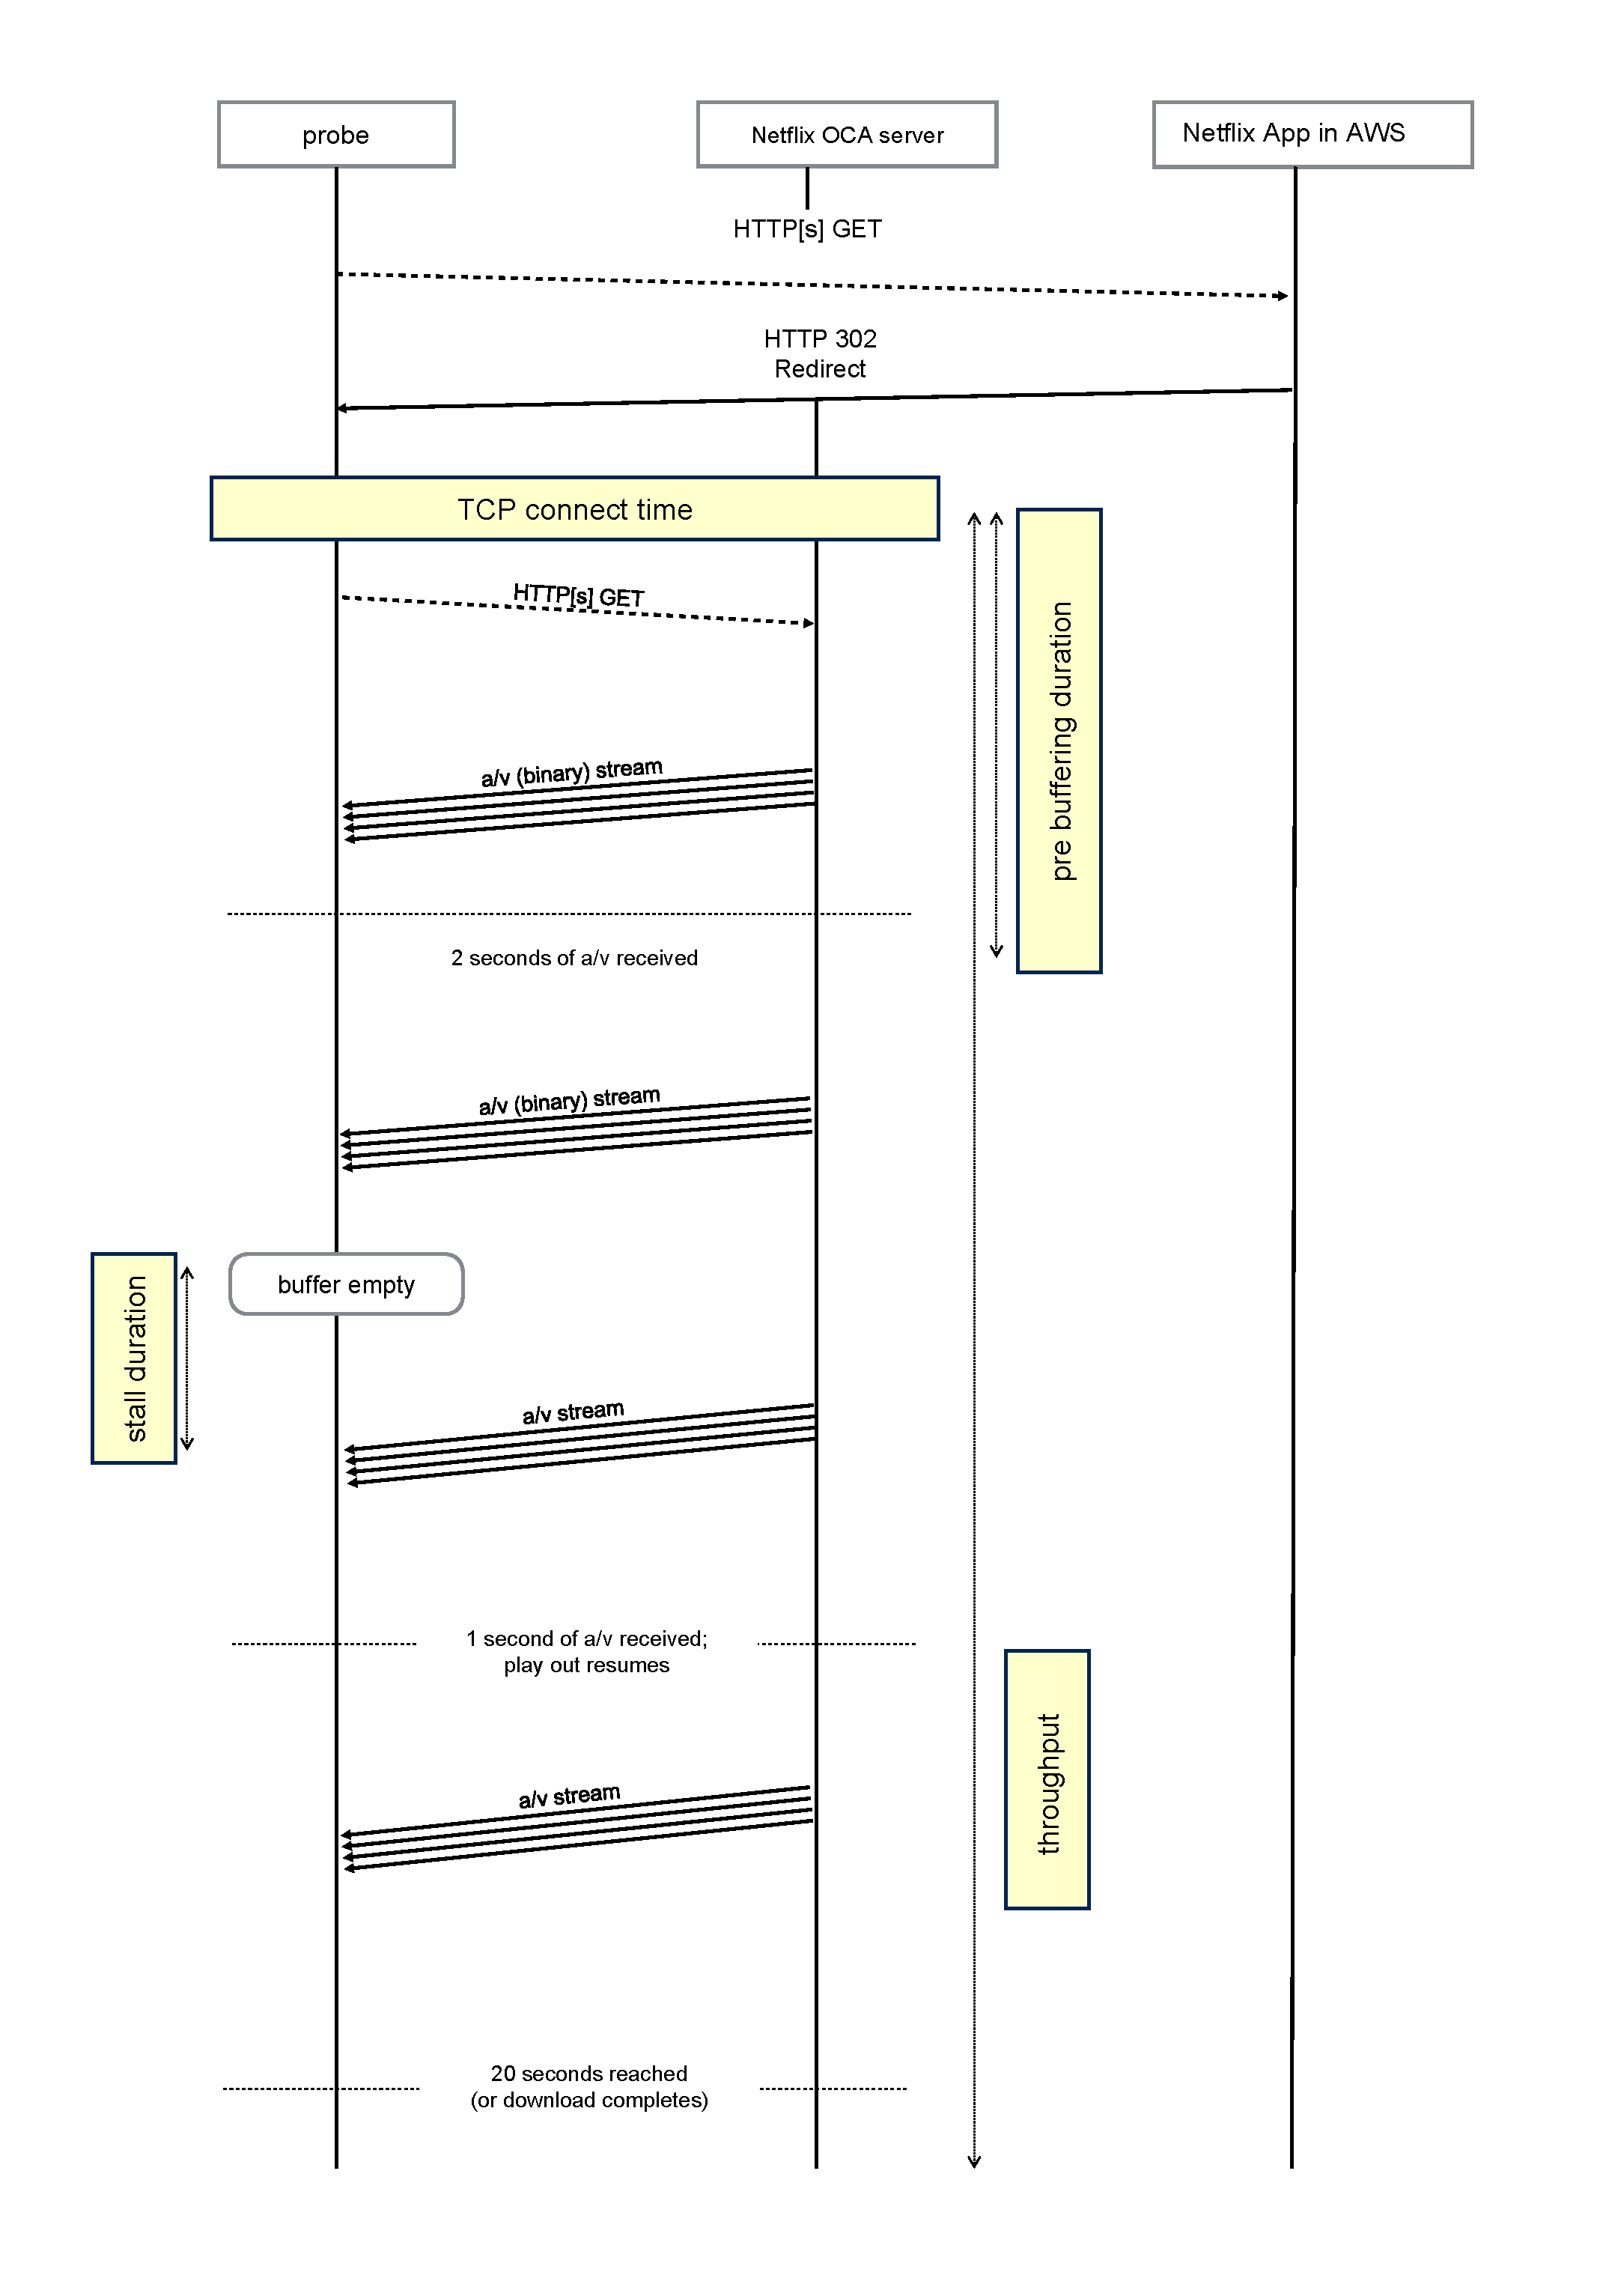
\includegraphics[keepaspectratio, height = 15cm, width=10cm]{figures/Netflix-Sequence-Diagram.pdf}
	\caption[Netflix Test Sequence Diagram]{A sequence diagram depicting the operation of the \texttt{netflix} test and the stages where different performance metrics are collected.}
	\label{fig:netflix test sequence diagram}
\end{figure}

Bajpai and Schönwälder in their study \cite{bajpaisurvey} explained the installation of SamKnows probes \cite{samknows}, 
which are hardware-based probes used to take Internet measurements. There are around 100 dual-stacked probes which are geographically deployed (refer \cref{fig:PROBES GEO DISTRIBUTION}) 
all over the world and are obtaining measurements over both IPv4 and IPv6. The probes are running hourly Paris-traceroute \cite{paris} measurements towards Netflix OCA servers using \textit{scamper} \cite{scamper}. 
SamKnows \cite{samknows} in direct cooperation with Netflix \cite{netflix} developed the Netflix Test, 
which is an application-specific test \cite{samknowswhitepaper}. The test measures the TCP Connect times, Prebuffering Duration, achieved throughput, the number of stalls and stall duration metrics
which help us evaluate the performance when streaming a Netflix video. The \cref{fig:netflix test sequence diagram} shows the sequence diagram of the operation of this Netflix test, it also
shows the stages where different performance metrics are collected. As per \cite{samknowswhitepaper} the \texttt{netflix} test is designed in such a way that it allows the streaming of binary data
from the Netflix OCA servers, also it uses the same OCA server selection logic as their real client uses when a registered user tries to access the content on their website. The functionality is
similar to what Netflix is using in \textit{Fast.com} \cite{fastcom}. Refer the official Netflix blog post related to the architecture of \textit{Fast.com} in \cite{netflixfast}. 

The explanation of the test is majorly based on \cite{samknowswhitepaper} and as per that the test starts by calling the Netflix web-based API which is hosted on AWS \cite{ocaoverview}.
Client source IP address, Traffic load, Network distance, and Location determines the selection of the OCA server, and the API provides this Netflix OCA server which will serve the content to the client.
This server can be a Netflix OCA server or can be an ISP content cache (if the ISP participates in Netflix OCA programme). The client receives an HTTP 302 redirect to a 25 MB binary file which is hosted on the Netflix OCA server, 
or on the ISP content cache.  After this, the client will connect to the received OCA server and will try to fetch the 25 MB binary file. The Netflix test runs for 20 seconds, and HTTP pipelining is used to fetch multiple copies of the binary file, which helps ensure receiving more data if the test runtime of 20 seconds is exhausted \cite{samknowswhitepaper}. 

Samknows \cite{samknowswhitepaper} further explains that the binary file is not an audio-video file, but with the knowledge of bitrates at which Netflix streams content, the binary data can be
treated as an audio-video data of a fixed bitrate. Furthermore, because of this, if there is a stall occurring, the download doesn't start again but the playback characteristics of the same network are simply recomputed at a different bitrate. The rest of the study explains the meaning of different metrics and the analysis we perform over those metrics.

\FloatBarrier

\section{Netflix Dataset Overview}\label{section:netflix-dataset}

\subsection*{\textit{Description}}

The Netflix dataset contains multiple tables (\textit{Netflix} and \textit{traceroute}), and each table consists of attributes which help us evaluate performance metrics such as \textit{Success Rate, Throughput, Error Rate, TCP Connect Times, Pre-Buffering Durations, Stall Rate, Path Length (TTL)} and so on.  The dataset collection was started from July 2016 and is running till date, so it's almost a two years dataset when this study got finished. The database consist of few tables which aren't relevant for this study and we haven't used them either, these are \textit{msmpoint}, \textit{netflix\_status}, and \textit{traceroute\_status}. The Netflix database can be found in /data/akapoor/netflix.db and the schema of the \textit{netflix} table is described in \cref{table:netflix}. 

\begin{table}[!h]
	\centering
	\caption{Schema of the \textit{Netflix} table}
	\label{table:netflix}
	\begin{tabular}{lp{11cm}}
  		\toprule
  		\textbf{Field} & \textbf{Description} \\ 
  		\midrule
  		unit\_id & The ID of the measurement probe \\ 
  		dtime & Timestamp (UTC) of the measurement as “YYYY–MM-DD HH:MM:SS” \\ 
		target & Netflix OCA hostname \\ 
		address &  Netflix OCA IP address \\ 
		bitrate & Bitrate of emulated video in bytes/sec \\ 
		max\_bitrate & The maximum bitrate supported by Netflix (currently always 15.6 Mbps) in bytes/sec \\ 
		stall\_events & How many times has it stalled at this bitrate \\  
		stall\_duration\_total & Sum off the durations (usec) of all the stalls \\ 
		connect\_time & Time it took to establish the TCP connection with the content server in usec \\ 
		download\_duration & Duration of the test in usec \\ 
		prebuffering\_duration &  How long it took to fetch 2 seconds of video at the specified bitrate in usec \\ 
		bytes\_sec  & Download speed in bytes/sec after the prebuffering finished \\ 
		error & Detailed error code \\ 
		error\_msg  &  Detailed error message if a problem occurred fetching the content from Netflix \\ 
		successes  & 1 if the test runs for the full duration (may have stalls though)   i.e. it was not aborted and stepped down \\ 
		failures  & 1 if the test was aborted for some reason \\
  		\bottomrule
\end{tabular}
\end{table}

\FloatBarrier

The \textit{error} and \textit{error\_msg} field in the \textit{netflix} table describes the errors and the their actual reasons for occurring. We have inferred the meanings of these errors from \textit{error\_msg} field and from our own research \cite{rfc2616} and \cite{httperror}. There are nine different kinds of errors including the "NO\_ERROR" value and \cref{table:errors} describes these errors and the possible reasons for their occurrence.

\begin{table}[!ht]
	\centering
	\caption{Overview of Errors (error and error\_msg field)}
	\label{table:errors}
	\begin{tabular}{lp{8cm}}
  		\toprule
  		\textbf{Error} & \textbf{Possible reasons} \\ 
  		\midrule
  		NO\_ERROR & The test was executed properly. \\ 
  		DNS\_RESOLUTION\_CONTENT\_ERROR & "getaddrinfo: Name or service not known", 
"getaddrinfo: ai\_family not supported", 
"getaddrinfo: Address family for hostname not supported", 
 \\ 
		DNS\_RESOLUTION\_API\_ERROR & "curl\_easy\_perform: Couldn't resolve host 'api-global.netflix.com'(IP:)", 
"curl\_easy\_perform: name lookup timed out (IP: )", 
 \\ 
		STALLED\_WILL\_STEP\_DOWN & When the client is configured to start testing at the highest supportable bitrate but step down to a lower bitrate when stalls occur. \\ 
		NETWORK\_CONTENT\_ERROR & "The speed was too low to finish the prebuffering"
"Server returned error 307", 
"recv: Connection reset by peer", 
"send: Resource temporarily unavailable", 
"Read timeout", 
"The server closed the connection", 
"Server returned error 500", 
"send: Broken pipe", 
 \\ 
		CONNECTION\_CONTENT\_ERROR & "Could not connect to host"
 \\ 
		NETWORK\_API\_ERROR & When there the server is not able to handle the requests (Error Code 503) or is temporarily unavailable (Error Code 500). Other reasons could be are connection timed out or operation timed out.  \\  
		CONNECTION\_API\_ERROR & When the Network is unreachable, or the client is not able to connect to the host.  \\ 
		STALLED\_ON\_FINAL & Stall happening for the lowest bitrate as well i.e. can’t step down after this. \\
  		\bottomrule
\end{tabular}
\end{table}

\FloatBarrier

As Viet \cite{viet} did in his thesis, we also created additional tables which assisted us in our study. 
We looked up the AS holder names from the RIPEstat \cite{ripestat} APIs for the respective destination i.e. \textit{address} field. We used the scripts by Bajpai et al. \cite{bajpairipe}, 
which were part of Measurement Research within the Python3 Ecosystem study. There are about 6000 distinct IP (both IPv4 and IPv6) addresses in the dataset and their AS holder names are depicted in \cref{table:asnname} and \cref{table:asn2name}. We further segregated this table for IPv4 and IPv6 and the results can be found in the \hyperref[chapter:appendix]{Appendices}.

\begin{table}[!h]
	\centering
	\caption{ASN Holder Names}
	\label{table:asnname}
	\begin{tabular}{lp{2cm}}
  		\toprule
  		\textbf{AS Name} & \textbf{\#IPs} \\ 
  		\midrule
		AS-SSI - Netflix Streaming Services Inc.      &                                  5612 \\
		BSKYB-BROADBAND-AS - Sky UK Limited             &                                  93 \\
		BT-UK-AS - British Telecommunications PLC       &                                  77 \\
		TELENOR-NEXTEL - Telenor Norge AS              &                                   60 \\
		TEKSAVVY - TekSavvy Solutions                 &                                    46 \\
		BELGACOM-SKYNET-AS - Proximus NV               &                                   43 \\
		EIRCOM - Eircom Limited                       &                                    14 \\
		GET-NO - Get AS                              &                                     14 \\
		COMHEM-SWEDEN - Com Hem AB                  &                                      13 \\
		XS4ALL-NL - Xs4all Internet BV              &                                      12 \\
		ALTIBOX\_AS - Altibox AS                         &                                  12 \\
		AS-VOBIZ - vanoppen.biz LLC                     &                                  12 \\
		PLUSNET - British Telecommunications PLC         &                                 12 \\
		INTERNODE-AS Internode Pty Ltd                   &                                 11 \\
		SNAP-NZ-AS Snap Internet Limited                 &                                 11 \\
		NEXTGENTEL - NextGenTel AS                       &                                 11 \\
		BEANFIELD - Beanfield Technologies Inc.          &                                 10 \\
		AUREON-5056 - Aureon Network Services            &                                 10 \\
		ALGAR TELECOM S/A                                &                                  8 \\
		SUNRISE - Sunrise Communications AG              &                                  8 \\
		ASBRUTELE - Brutele SC                           &                                  8 \\
		BREDBAND2 - Bredband2 AB                         &                                  7 \\
		ALLST-15290 - Allstream Corp.                    &                                  6 \\
		ASN-CATCHCOM - Broadnet AS                       &                                  6 \\
		CALLPLUS-NZ-AP CallPlus Services Limited          &                                 5 \\
		RCN-AS - RCN                                        &                               5 \\
		MOBILEONELTD-AS-AP MobileOne Ltd.   &     4 \\
		\bottomrule
\end{tabular}
\end{table}

\begin{table}[!h]
	\centering
	\caption{Continuing \cref{table:asnname}}
	\label{table:asn2name}
	\begin{tabular}{lp{2cm}}
  		\toprule
  		\textbf{AS Name} & \textbf{\#IPs} \\ 
  		\midrule
		MNET-AS - M-net Telekommunikations GmbH                                &            4 \\
		INIT7 - Init7 (Switzerland) Ltd.                               &                    4 \\
		NORDUNET - NORDUnet                                      &                          4 \\
		PENNREN - KINBER                                        &                           4 \\
		CENTURYLINK-US-LEGACY-QWEST - Qwest Comm. Co.    &                    3 \\
		WAIA-TRANSIT-AP Western Australian Internet Association     &                       3 \\
		UUNET - MCI Communications Services           &                                    3 \\
		TEKSAVVY-WEST - TekSavvy Solutions             &                                    2 \\
		ASN-IINET iiNet Limited                        &                                    2 \\
		TPG-INTERNET-AP TPG Telecom Limited              &                                  2 \\
		PREMIER-COMMUNICATIONS - Premier Communications       &                             2 \\
		EWETEL - EWE TEL GmbH                                 &                             2 \\
		NMAX - Nmax                                            &                            1 \\
		ASSOCIAÇÃO NACIONAL PARA INCLUSÃO DIGITAL - ANID        &                           1 \\
		PSC-EXT - Pittsburgh Supercomputing Center              &                           1 \\
		T-MOBILE-AS21928 - T-Mobile USA                      &                              1 \\
		WEBFOCO TELECOMUNICACOES LTDA                        &                              1 \\
		G8 NETWORKS LTDA                                      &                             1 \\
		TBNet Informatica LTDA                                &                             1 \\
		Rede Connect Telecom                                  &                             1 \\
  		\bottomrule
\end{tabular}
\end{table}

\FloatBarrier

The Netflix dataset has the \textit{traceroute} table which consists of TTL and RTTs values to the Netflix CDN hosts. The schema of the \textit{traceroute} table can be found in \cref{table:traceroute}.  

\begin{table}[!h]
	\centering
	\caption{Schema of the \textit{traceroute and traceroute-filtered} table}
	\label{table:traceroute}
	\begin{tabular}{lp{10cm}}
  		\toprule
  		\textbf{Field} & \textbf{Description} \\ 
  		\midrule
  		unit\_id & The ID of the measurement probe \\ 
  		dtime & Timestamp (UTC) as “YYYY–MM-DD HH:MM:SS” \\ 
		version & Scamper version used for the measurement \\ 
		source &  IP address of the source \\ 
		destination & IP address of the destination \\ 
		method & Traceroute variant \\ 
		status & Measurement status \\  
		ttl & TTL of the packet \\ 
		endpoint & IP address of the intermediate hop \\
		rtt & RTT of the packet \\
  		\bottomrule
\end{tabular}
\end{table}

\FloatBarrier

The status column in the above table tells us whether a measurement was completed or not. It also defines the reasons if the measurement was not completed. 
The possible reasons are depicted in \cref{table:status} and their meanings were inferred from the
dataset and from our own research about scamper \cite{status1}, and \cite{status2}.

\begin{table}[!h]
	\centering
	\caption{Overview of possible stop reasons (status values) for scamper}
	\label{table:status}
	\begin{tabular}{lp{7cm}}
  		\toprule
  		\textbf{Reasons} & \textbf{Description} \\ 
  		\midrule
  		COMPLETED & Destination reached, traceroute measurement successful \\
  		GAPLIMIT & Destination reached, traceroute measurement successful \\
		UNREACH & ICMP destination unreachable message received \\
		LOOP & Specific IP address appeared twice in the same trace \\
		ERROR & Error occurred when sending messages on socket (sendto() error) \\
  		\bottomrule
\end{tabular}
\end{table}

\FloatBarrier

We further followed the same approach of aggregation which Viet followed in his Master's Thesis \cite{viet}. Therefore, most of the table described below are based on his work. 
We collected the public source IPs of the probes from the SamKnows \cite{samknows} dashboard and queried the RIPEstat \cite{ripestat} API to get the AS number and holder name for these public \textit{source} IPs, \textit{endpoint} IPs, and \textit{destination} IPs. The public source IPs we collected can be found at /metadata/sources.csv and we were only able to collect the IPv4 addresses. We used the IPv6 addresses available from the \textit{traceroute} table. The resulted tables can be found in table \cref{table:destination}, \cref{table:source}, and \cref{table:endpoint}. 

\begin{table}[!h]
	\centering
	\caption{Schema of the \textit{dst\_asn\_mapping} table}
	\label{table:destination}
	\begin{tabular}{lp{7cm}}
  		\toprule
  		\textbf{Field} & \textbf{Description} \\ 
  		\midrule
  		ip & IP address of the destination \\
  		asn & AS Number of the Source \\
  		holder & Entity name which owns the AS \\
  		\bottomrule
\end{tabular}
\end{table}

\begin{table}[!h]
	\centering
	\caption{Schema of the \textit{src\_asn\_mapping} table}
	\label{table:source}
	\begin{tabular}{lp{7cm}}
  		\toprule
  		\textbf{Field} & \textbf{Description} \\ 
  		\midrule
  		unit\_id & The ID of the measurement probe \\
  		src\_ip & Public IP address of the source \\
  		asn & AS Number of the Source \\
  		holder & Entity name which owns the AS \\
  		\bottomrule
\end{tabular}
\end{table}

\begin{table}[!h]
	\centering
	\caption{Schema of the \textit{endpoint\_asn\_mapping} table}
	\label{table:endpoint}
	\begin{tabular}{lp{7cm}}
  		\toprule
  		\textbf{Field} & \textbf{Description} \\ 
  		\midrule
  		endpoint & Endpoint or Intermediate hop IP address \\
  		asnnum & AS Number of the Endpoint \\
  		holder & Entity name which owns the AS \\
  		\bottomrule
\end{tabular}
\end{table}

\FloatBarrier

We wanted to find out the AS type for the individual endpoints along the destination paths. CAIDA \cite{caida} does classify every AS according to three types i.e. \textit{Transit, Content, and Enterprise}. These CAIDA  classifications are based on their machine learning algorithm and the PeeringDB classifications \cite{peeringdb}; \cref{table:caida} contains the schema for the CAIDA dataset.    

\begin{table}[!h]
	\centering
	\caption{Schema of the \textit{as\_types} table}
	\label{table:caida}
	\begin{tabular}{lp{7cm}}
  		\toprule
  		\textbf{Field} & \textbf{Description} \\ 
  		\midrule
  		asn & AS number, assigned by Internet Assigned Numbers Authority (IANA)\\
  		source & Used classifier i.e. CAIDA\_class or peerDB\_class \\
  		type & Business type of the AS \\
  		\bottomrule
\end{tabular}
\end{table}

\FloatBarrier

Reverse DNS lookup of the destination IPs are contained in \cref{table:hostnames}, to help us further classify the IPs. We again used RIPEstat \cite{ripestat} to  get this information, and as result table \textit{hostnames} is created. 
Although there are around 6689 destination IPs only 5154 IPs could be looked up. 

\begin{table}[!h]
	\centering
	\caption{Schema of the \textit{hostnames} table}
	\label{table:hostnames}
	\begin{tabular}{lp{7cm}}
  		\toprule
  		\textbf{Field} & \textbf{Description} \\ 
  		\midrule
  		ip & IP address of the destination \\
  		hostname & Reverse DNS hostname \\
  		\bottomrule
\end{tabular}
\end{table}

\FloatBarrier

\subsection*{Aggregation}

We aggregated the original \textit{traceroute} table to help us in our analysis. Our motivation for doing this aggregation was to get a detailed overview of the dataset and to avoid unnecessary repetition of steps required for dataset filtering. All the below-mentioned tables were pushed onto the same database i.e. at /data/akapoor/netflix.db. We will briefly explain the steps that we followed in this aggregation and filtering. As already informed, we followed the same strategy that Viet \cite{viet} followed in his study. The reason for this is that Viet used the \textit{Youtube} dataset which has the similar schema as \textit{Netflix} dataset, and both datasets are collected using SamKnows probes \cite{samknows}. 


We started out by filtering the \textit{traceroute} table, and we first removed 
the rows which contained NaN values or the probes which don't contain 
measurements for both the IP address families i.e probes with \textit{unit\_id} 
525884 and 658929. We further removed measurements from Hurricane Electric Probes 
(refer \cite{he1}, \cite{he2}, \cite{he3}, \cite{he4} and \cite{he5}), due to the reasons discussed in chapter \textit{Related Work}. Therefore, we removed the rows which contained measurements from probes which belonged to Hurricane Electric i.e. AS 6939 (refer \cref{table:source} for such probes). The dataset contains a lot of duplicated rows, originated due to various reasons and we had to drop these rows to remove redundancy. The original \textit{traceroute} table had 34002477 rows and after performing all these operations the rows were reduced to 8768279. We named the resulting table \textit{traceroute-filtered} which contains the non-duplicate rows with measurements from dual-stacked probes only, and its schema is depicted in \cref{table:traceroute}. 


We used an additional table which we didn't explicitly pushed to our database, but it contains the \textit{COMPLETED} i.e. status == 'COMPLETED' results (refer \cref{table:status} for more information). 
We named this table \textit{completed-traceroute} and it contains the whole TTL measurements i.e. where TTL increments by one for the desired path sequence. 
We further rounded the \textit{dtime} field to hours and dropped the columns which were not relevant for our analysis. The schema for the \textit{completed-traceroute} table can be found in \cref{table:completed}. 

\begin{table}[!h]
	\centering
	\caption{Schema of \textit{completed-traceroute} table}
	\label{table:completed}
	\begin{tabular}{lp{8cm}}
  		\toprule
  		\textbf{Field} & \textbf{Description} \\ 
  		\midrule
  		unit\_id & The ID of the measurement probe \\ 
  		dtime & Timestamp (UTC) of the measurement as “YYYY–MM-DD HH:00:00” \\  
		source &  IP address of the source \\ 
		destination & IP address of the destination \\   
		ttl & TTL for this path \\ 
		rtt & RTT of the packet \\
  		\bottomrule
\end{tabular}
\end{table}

\FloatBarrier

After considering the "COMPLETED" results, we further filtered the data based on matching IP addresses in the \textit{destination} and \textit{endpoint} fields. We then selected the maximum TTL values based on the grouping of \textit{unit\_id, dtime, source and destination} fields, as done by Viet \cite{viet}. We did this filtering to make sure that we only analyze the traceroute results which were completed and actually reached the destination. Also, multiple rows for a single path were reduced to only one row with the maximum TTL value and the RTT value for the whole path. The grouping fields that we selected above ensures to filter only one traceroute measurement per path i.e. for a specific \textit{source} and a \textit{destination}. 

We split-up this table for IPv4 and IPv6 addresses and the schema for these tables are depicted in \cref{table:traceroutev4v6}.

\begin{table}[!h]
	\centering
	\caption{Schema of \textit{traceroute\_v4 and traceroute\_v6} tables}
	\label{table:traceroutev4v6}
	\begin{tabular}{lp{8cm}}
  		\toprule
  		\textbf{Field} & \textbf{Description} \\ 
  		\midrule
  		unit\_id & The ID of the measurement probe \\ 
  		dtime & Timestamp (UTC) of the measurement as “YYYY–MM-DD HH:MM:SS” \\  
		source &  IP address of the source \\ 
		destination & IP address of the destination \\   
		max(ttl) & Maximum TTL for this path \\ 
		rtt & RTT of the packet \\
  		\bottomrule
\end{tabular}
\end{table}

\FloatBarrier

To further compare the two address family's i.e. IPv4 and IPv6, we merged both the tables \cref{table:traceroutev4v6}. As the data was collected every hour, concurrently for IPv4 and IPv6, \textit{unit\_id and dtime} could be used to identify traceroute measurements pairs for both the address families. 

We rounded the time in \textit{traceroute\_v4} and \textit{traceroute\_v6} to nearest hour, to identify such measurement pairs. After doing this, we then merged the two tables group by \textit{unit\_id} and \textit{dtime(rounded)} fields, and computed the deltas for the max(TTL) and RTT fields. The resulting schema can be found in \cref{table:deltas}, where fields with the same description are shown side-by-side.

\begin{table}[!h]
	\centering
	\caption{Schema of \textit{deltas} table (difference of \textit{traceroute\_v4} and \textit{traceroute\_v6} tables)}
	\label{table:deltas}
	\begin{tabular}{lp{8cm}}
  		\toprule
  		\textbf{Field} & \textbf{Description} \\ 
  		\midrule
  		unit\_id & The ID of the measurement probe \\ 
  		dtime & Timestamp (UTC) of the measurement as “YYYY–MM-DD HH:MM:SS” \\  
		source\_v4 and source\_v6 &  IP address of the source \\ 
		destination\_v4 and destination\_v6 & IP address of the destination \\   
		max(ttl)\_v4 and max(ttl)\_v6 & Maximum TTL for this path \\ 
		rtt\_v4 and rtt\_v6 & RTT of the packet \\
		ttl\_delta & $\Delta$TTL \\
		rtt\_delta & $\Delta$RTT \\
  		\bottomrule
\end{tabular}
\end{table}

\FloatBarrier

We wanted to analyze data irrespective of the time, and therefore we removed the \textit{dtime} field to achieve this. The \textit{traceroute\_v4 and traceroute\_v6} tables were further grouped by \textit{unit\_id, source, and destination} fields, which denote recurring paths from the source IP address to the destination IP address for the whole period, and we computed the median TTL and median RTT values for this group. The tables \textit{path\_medians\_v4} and \textit{path\_medians\_v6} achieved after this operation are shown in \cref{table:pathv4v6}. 

\begin{table}[!h]
	\centering
	\caption{Schema of \textit{path\_medians\_v4 and path\_medians\_v6} tables}
	\label{table:pathv4v6}
	\begin{tabular}{lp{7cm}}
  		\toprule
  		\textbf{Field} & \textbf{Description} \\ 
  		\midrule
  		unit\_id & The ID of the measurement probe \\ 
		source &  IP address of the source \\ 
		destination & IP address of the destination \\   
		median(ttl) & Median TTL for this path \\ 
		median(rtt) & Median RTT of the packet \\
  		\bottomrule
\end{tabular}
\end{table}

\FloatBarrier

The \textit{deltas} table was also filtered and we removed the \textit{dtime} field to analyze the data irrespective of the time factor. We considered the \textit{unit\_id, destination\_v4, and destination\_v6} grouping to achieve the measurements pairs and calculated the median TTL and median RTT for these measurement pairs. We further calculated the deltas for the median TTL and median RTT, and the resulting schema can be seen in \cref{table:pair}.  

\begin{table}[!h]
	\centering
	\caption{Schema of \textit{pair\_medians} table}
	\label{table:pair}
	\begin{tabular}{lp{7cm}}
  		\toprule
  		\textbf{Field} & \textbf{Description} \\ 
  		\midrule
  		unit\_id & The ID of the measurement probe \\ 
		source\_v4 and source\_v6 &  IP address of the source \\ 
		destination\_v4 and destination\_v6 & IP address of the destination \\   
		max(ttl)\_v4 and max(ttl)\_v6 & Median TTL for this path \\ 
		rtt\_v4 and rtt\_v6 & Median RTT of the packet \\
		ttl\_delta & Median $\Delta$TTL \\
		rtt\_delta & Median $\Delta$RTT \\
  		\bottomrule
\end{tabular}
\end{table}

\FloatBarrier

We further created a table containing the metadata from the additional tables \cref{table:destination}, \cref{table:source}, and  \cref{table:hostnames}. The ASN mappings were joined based on an inner join, and the reverse DNS lookup hostnames were joined based on an outer join. Here, the measurements from probes with no public source IP were dropped due to the inner join. The resulting table is \textit{pair\_medians\_meta} and the schema can be found in \cref{table:pairmeta}.  

\begin{table}[!h]
	\centering
	\caption{Schema of \textit{pair\_medians\_meta} table}
	\label{table:pairmeta}
	\begin{tabular}{lp{8cm}}
  		\toprule
  		\textbf{Field} & \textbf{Description} \\ 
  		\midrule
  		unit\_id & The ID of the measurement probe \\ 
		src\_v4 and src\_v6 &  IP address of the source \\
		src\_asn\_v4 and src\_asn\_v6 & AS Number of the Source IP address \\
		src\_holder\_v4 and src\_holder\_v6 & Entity owning the AS number \\ 
		dst\_v4 and dst\_v6 & IP address of the destination \\
		hostname\_v4 and hostname\_v6 & Hostname of destination \\ 
		dst\_asn\_v4 and dst\_asn\_v6 & AS Number of the Destination IP address \\
		dst\_holder\_v4 and dst\_holder\_v6 & Entity owning the AS number  \\
		m\_ttl\_v4 and m\_ttl\_v6 & Median TTL to reach the destination \\ 
		m\_rtt\_v4 and m\_rtt\_v6 & Median RTT of the packet \\
		m\_ttl\_delta & Median $\Delta$TTL \\
		m\_rtt\_delta & Median $\Delta$RTT \\
  		\bottomrule
\end{tabular}
\end{table}

\FloatBarrier

\section{SpeedTest Dataset Overview}

\subsection*{Description}

We further investigated and analyzed the Speedtest dataset which is measurements of metrics towards Measurement Lab servers, therefore we will call it M-Lab Dataset from now onwards. Similar to Netflix, the M-Lab dataset also contains tables which help us evaluate the \textit{throughput and TTL} measurements. We will compare the performance of both Netflix and M-Lab servers, and the dataset collection was started in September 2014 and is running till date. 
The dataset consists of few tables which aren't relevant to this study, these are namely \textit{httppostmt, httppostmt6, httpgetmt\_status, httpgetmt6\_status, httppostmt, httppostmt6\_status, msmpoint, and traceroute\_status}. The M-lab dataset can be found at /data/akapoor/speedtest.db and the schema of the used tables are mentioned below. Note, we aren't specifying all the fields present in the table, but only the ones we are using for our analysis to maintain readability and context. The \textit{httpgetmt and httpgetmt6} tables are used to compare the throughput of M-Lab media servers with Netflix OCA servers. Here, the relevant field is \textit{bytes\_sec}, and the schema can be found in \cref{table:mlabv4} and \cref{table:mlabv6} for IPv4 and IPv6 address family's respectively.

\begin{table}[!h]
	\centering
	\caption{Schema of the \textit{httpgetmt} table}
	\label{table:mlabv4}
	\begin{tabular}{lp{10cm}}
  		\toprule
  		\textbf{Field} & \textbf{Description} \\ 
  		\midrule
  		unit\_id & The ID of the measurement probe \\ 
  		dtime & Timestamp (UTC) of the measurement as “YYYY–MM-DD HH:MM:SS” \\ 
		target & M-Lab IPv4 hostname \\ 
		address &  M-Lab IPv4 address \\ 
		bytes\_sec  & Download speed in bytes/sec after the prebuffering finished \\  
		successes  & 1 if the test runs for the full duration (may have stalls though) i.e. it was not aborted and stepped down \\ 
		failures  & 1 if the test was aborted for some reason \\
  		\bottomrule
\end{tabular}
\end{table}

\begin{table}[!h]
	\centering
	\caption{Schema of the \textit{httpgetmt6} table}
	\label{table:mlabv6}
	\begin{tabular}{lp{10cm}}
  		\toprule
  		\textbf{Field} & \textbf{Description} \\ 
  		\midrule
  		unit\_id & The ID of the measurement probe \\ 
  		dtime & Timestamp (UTC) of the measurement as “YYYY–MM-DD HH:MM:SS” \\ 
		target & M-Lab IPv6 hostname \\ 
		address &  M-Lab IPv6 address \\ 
		bytes\_sec  & Download speed in bytes/sec after the prebuffering finished \\  
		successes  & 1 if the test runs for the full duration (may have stalls though) i.e. it was not aborted and stepped down \\ 
		failures  & 1 if the test was aborted for some reason \\
  		\bottomrule
\end{tabular}
\end{table}

\FloatBarrier

We also wanted to compare the path lengths of Netflix and M-Lab for the corresponding throughputs, thus we used the M-Lab's \textit{traceroute} table for this. Note here that we are following the same strategy \cite{viet} did in his study and thus, the following tables and aggregation is based on his work. Also to note, as we already explained these tables and aggregation strategy in \cref{section:netflix-dataset}. Therefore, the reader can skip the following section as it provides the same description and information. 

The M-Lab dataset has the \textit{traceroute} table which consists of TTL and RTTs values to the M-Lab media servers. The traceroute measurements were started in May 2016 and are running till date. The schema of the \textit{traceroute} table can be found in \cref{table:traceroutemlab}.

\begin{table}[!h]
	\centering
	\caption{Schema of the \textit{traceroute and traceroute-filtered} table}
	\label{table:traceroutemlab}
	\begin{tabular}{lp{10cm}}
  		\toprule
  		\textbf{Field} & \textbf{Description} \\ 
  		\midrule
  		unit\_id & The ID of the measurement probe \\ 
  		dtime & Timestamp (UTC) of the measurement as “YYYY–MM-DD HH:MM:SS” \\ 
		version & Scamper version used for the measurement \\ 
		source &  IP address of the source \\ 
		destination & IP address of the destination \\ 
		method & Traceroute variant \\ 
		status & Measurement status \\  
		ttl & TTL of the packet \\ 
		endpoint & IP address of the intermediate hop \\
		rtt & RTT of the packet \\
		location\_id & Internal ID denoting geographical location of the probe \\
  		\bottomrule
\end{tabular}
\end{table}

\FloatBarrier

We collected the public source IPs of the probes from the SamKnows \cite{samknows} dashboard and queried the RIPEstat \cite{ripestat} API to get the AS number and holder name for these public \textit{source} IPs, \textit{endpoint} IPs, and \textit{destination} IPs. The public source IPs we collected can be found at /metadata/sources.csv and we were only able to collect the IPv4 addresses. We used the IPv6 addresses available from the \textit{traceroute} table. The resulted M-Lab tables can be found in \cref{table:destinationmlab}, \cref{table:sourcemlab}, and \cref{table:endpointmlab}.

\begin{table}[!h]
	\centering
	\caption{Schema of the \textit{dst\_asn\_mapping} table}
	\label{table:destinationmlab}
	\begin{tabular}{lp{7cm}}
  		\toprule
  		\textbf{Field} & \textbf{Description} \\ 
  		\midrule
  		ip & IP address of the destination \\
  		asn & AS Number of the Source \\
  		holder & Entity name which owns the AS \\
  		\bottomrule
\end{tabular}
\end{table}

\begin{table}[!h]
	\centering
	\caption{Schema of the \textit{src\_asn\_mapping} table}
	\label{table:sourcemlab}
	\begin{tabular}{lp{7cm}}
  		\toprule
  		\textbf{Field} & \textbf{Description} \\ 
  		\midrule
  		unit\_id & The ID of the measurement probe \\
  		src\_ip & Public IP address of the source \\
  		asn & AS Number of the Source \\
  		holder & Entity name which owns the AS \\
  		\bottomrule
\end{tabular}
\end{table}

\begin{table}[!h]
	\centering
	\caption{Schema of the \textit{endpoint\_asn\_mapping} table}
	\label{table:endpointmlab}
	\begin{tabular}{lp{7cm}}
  		\toprule
  		\textbf{Field} & \textbf{Description} \\ 
  		\midrule
  		endpoint & Endpoint or Intermediate hop IP address \\
  		asnnum & AS Number of the Endpoint \\
  		holder & Entity name which owns the AS \\
  		\bottomrule
\end{tabular}
\end{table}

\FloatBarrier

We wanted to find out the AS type for the individual endpoints along the destination paths. CAIDA \cite{caida} does classify every AS according to three types i.e. \textit{Transit, Content, and Enterprise}. These CAIDA classifications are based on their machine learning algorithm and the PeeringDB classifications \cite{peeringdb}; \cref{table:caidamlab} contains the schema for the CAIDA dataset.

\begin{table}[!h]
	\centering
	\caption{Schema of the \textit{as\_types} table}
	\label{table:caidamlab}
	\begin{tabular}{lp{7cm}}
  		\toprule
  		\textbf{Field} & \textbf{Description} \\ 
  		\midrule
  		asn & AS number, assigned by Internet Assigned Numbers Authority (IANA)\\
  		source & Used classifier i.e. CAIDA\_class or peerDB\_class \\
  		type & Business type of the AS \\
  		\bottomrule
\end{tabular}
\end{table}

\FloatBarrier

Reverse DNS lookup of the destination IPs of the M-Lab media servers are contained in \cref{table:hostnamesmlab}, to help us further classify the IPs. We again used RIPEstat \cite{ripestat} to get this information, and as result table \textit{hostnames} is created. Although there are around 158 destination IPs only 45 IPs could be looked up.

\begin{table}[!h]
	\centering
	\caption{Schema of the \textit{hostnames} table}
	\label{table:hostnamesmlab}
	\begin{tabular}{lp{7cm}}
  		\toprule
  		\textbf{Field} & \textbf{Description} \\ 
  		\midrule
  		ip & IP address of the destination \\
  		hostname & Reverse DNS hostname \\
  		\bottomrule
\end{tabular}
\end{table}

\FloatBarrier

\subsection*{Aggregation}

We aggregated the original \textit{traceroute} table to help us in our analysis. Our motivation for doing this aggregation was to get a detailed overview of the dataset and to avoid unnecessary repetition of steps required for dataset filtering. All the below-mentioned tables were pushed onto the same database i.e. at /data/akapoor/speedtest.db. We will briefly explain the steps that we followed in this aggregation and filtering. As already informed, we followed the same strategy that Viet \cite{viet} followed in his study. The reason for this is that Viet used the \textit{Youtube} dataset which has the similar schema as \textit{M-Lab} dataset, and both datasets are collected using SamKnows probes \cite{samknows}. 


We started out by filtering the \textit{traceroute} table, we first removed the rows which contained NaN values or the probes which don't contain measurements for both the IP address families i.e probes with \textit{unit\_id} 525884 and 658929. We further removed measurements from Hurricane Electric Probes (refer \cite{he1}, \cite{he2}, \cite{he3}, \cite{he4}, and \cite{he5}), due to the reasons discussed in chapter \textit{Related Work}. Therefore, we removed the rows which contained measurements from probes which belonged to Hurricane Electric i.e. AS 6939 (refer \cref{table:source} for such probes). The dataset contains a lot of duplicated rows, originated due to various reasons and we had to drop these rows to remove redundancy. The original \textit{traceroute} table had 12365994 rows and after performing all these operations the rows were reduced to 3522311. We named the resulting table \textit{traceroute-filtered} which contains the non-duplicate rows with measurements from dual-stacked probes only, and its schema is depicted in \cref{table:traceroutemlab}. 


We used an additional table which we didn't explicitly pushed to our database, but it contains the \textit{COMPLETED} i.e. status == 'COMPLETED' results (refer \cref{table:statusmlab} for more information). We named this table \textit{completed-traceroute} and it contains the whole TTL measurements i.e. where TTL increments by one for the desired path sequence. We further rounded the \textit{dtime} field to hours and dropped the columns which were not relevant for our analysis. The schema for the \textit{completed-traceroute} table can be found in \cref{table:completedmlab}. 

\begin{table}[!h]
	\centering
	\caption{Schema of \textit{completed-traceroutemlab} table}
	\label{table:completedmlab}
	\begin{tabular}{lp{8cm}}
  		\toprule
  		\textbf{Field} & \textbf{Description} \\ 
  		\midrule
  		unit\_id & The ID of the measurement probe \\ 
  		dtime & Timestamp (UTC) of the measurement as “YYYY–MM-DD HH:00:00” \\  
		source &  IP address of the source \\ 
		destination & IP address of the destination \\   
		ttl & TTL for this path \\ 
		rtt & RTT of the packet \\
  		\bottomrule
\end{tabular}
\end{table}

\FloatBarrier

After considering the "COMPLETED" results, we further filtered the data based on matching IP addresses in the \textit{destination} and \textit{endpoint} fields. We then selected the maximum TTL values based on the grouping of \textit{unit\_id, dtime, source and destination} fields, as done by Viet \cite{viet}. We did this filtering to make sure that we only analyze the traceroute results which were completed and actually reached the destination. Also, multiple rows for a single path were reduced to only one row with the maximum TTL value and the RTT value for the whole path. The grouping fields that we selected above ensures to filter only one traceroute measurement per path i.e. for a specific \textit{source} and a \textit{destination}. 

We split-up this table for IPv4 and IPv6 addresses and the schema for these tables are depicted in \cref{table:traceroutev4v6mlab}.

\begin{table}[!h]
	\centering
	\caption{Schema of \textit{traceroute\_v4 and traceroute\_v6} tables}
	\label{table:traceroutev4v6mlab}
	\begin{tabular}{lp{8cm}}
  		\toprule
  		\textbf{Field} & \textbf{Description} \\ 
  		\midrule
  		unit\_id & The ID of the measurement probe \\ 
  		dtime & Timestamp (UTC) of the measurement as “YYYY–MM-DD HH:MM:SS” \\  
		source &  IP address of the source \\ 
		destination & IP address of the destination \\   
		max(ttl) & Maximum TTL for this path \\ 
		rtt & RTT of the packet \\
  		\bottomrule
\end{tabular}
\end{table}

\FloatBarrier

To further compare the two address family's i.e. IPv4 and IPv6, we merged both the tables \cref{table:traceroutev4v6mlab}. As the data was collected every hour, concurrently for IPv4 and IPv6, \textit{unit\_id and dtime} could be used to identify traceroute measurements pairs for both the address families. 

We rounded the time in \textit{traceroute\_v4} and \textit{traceroute\_v6} to nearest hour, to identify such measurement pairs. After doing this, we then merged the two tables group by \textit{unit\_id} and \textit{dtime(rounded)} fields, and computed the deltas for the max(TTL) and RTT fields. The resulting schema can be found in \cref{table:deltasmlab}, where fields with the same description are shown side-by-side.

\begin{table}[!h]
	\centering
	\caption{Schema of \textit{deltas} table (difference of \textit{traceroute\_v4} and \textit{traceroute\_v6} tables)}
	\label{table:deltasmlab}
	\begin{tabular}{lp{8cm}}
  		\toprule
  		\textbf{Field} & \textbf{Description} \\ 
  		\midrule
  		unit\_id & The ID of the measurement probe \\ 
  		dtime & Timestamp (UTC) of the measurement as “YYYY–MM-DD HH:MM:SS” \\  
		source\_v4 and source\_v6 &  IP address of the source \\ 
		destination\_v4 and destination\_v6 & IP address of the destination \\   
		max(ttl)\_v4 and max(ttl)\_v6 & Maximum TTL for this path \\ 
		rtt\_v4 and rtt\_v6 & RTT of the packet \\
		ttl\_delta & $\Delta$TTL \\
		rtt\_delta & $\Delta$RTT \\
  		\bottomrule
\end{tabular}
\end{table}

\FloatBarrier

We wanted to analyze data irrespective of the time, and therefore we removed the \textit{dtime} field to achieve this. The \textit{traceroute\_v4 and traceroute\_v6} tables were further grouped by \textit{unit\_id, source, and destination} fields, which denote recurring paths from the source IP address to the destination IP address for the whole period, and we computed the median TTL and median RTT values for this group. The tables \textit{path\_medians\_v4} and \textit{path\_medians\_v6} achieved after this operation are shown in \cref{table:pathv4v6mlab}.

\begin{table}[!h]
	\centering
	\caption{Schema of \textit{path\_medians\_v4 and path\_medians\_v6} tables}
	\label{table:pathv4v6mlab}
	\begin{tabular}{lp{7cm}}
  		\toprule
  		\textbf{Field} & \textbf{Description} \\ 
  		\midrule
  		unit\_id & The ID of the measurement probe \\ 
		source &  IP address of the source \\ 
		destination & IP address of the destination \\   
		median(ttl) & Median TTL for this path \\ 
		median(rtt) & Median RTT of the packet \\
  		\bottomrule
\end{tabular}
\end{table}

\FloatBarrier

The \textit{deltas} table was also filtered and we removed the \textit{dtime} field to analyze the data irrespective of the time factor. We considered the \textit{unit\_id, destination\_v4, and destination\_v6} grouping to achieve the measurements pairs and calculated the median TTL and median RTT for these measurement pairs. We further calculated the deltas for the median TTL and median RTT, and the resulting schema can be seen in \cref{table:pairmlab}.  

\begin{table}[!h]
	\centering
	\caption{Schema of \textit{pair\_medians} table}
	\label{table:pairmlab}
	\begin{tabular}{lp{7cm}}
  		\toprule
  		\textbf{Field} & \textbf{Description} \\ 
  		\midrule
  		unit\_id & The ID of the measurement probe \\ 
		source\_v4 and source\_v6 &  IP address of the source \\ 
		destination\_v4 and destination\_v6 & IP address of the destination \\   
		max(ttl)\_v4 and max(ttl)\_v6 & Median TTL for this path \\ 
		rtt\_v4 and rtt\_v6 & Median RTT of the packet \\
		ttl\_delta & Median $\Delta$TTL \\
		rtt\_delta & Median $\Delta$RTT \\
  		\bottomrule
\end{tabular}
\end{table}

\FloatBarrier

We created a table containing the metadata from the additional tables \cref{table:destinationmlab}, \cref{table:sourcemlab}, and \cref{table:hostnamesmlab}. The ASN mappings were joined based on an inner join, and the reverse DNS lookup hostnames were joined based on an outer join. Here, the measurements from probes with no public source IP were dropped due to the inner join. The resulting table is \textit{pair\_medians\_meta} and the schema can be found in \cref{table:pairmetamlab}.  

\begin{table}[!h]
	\centering
	\caption{Schema of \textit{pair\_medians\_meta} table}
	\label{table:pairmetamlab}
	\begin{tabular}{lp{8cm}}
  		\toprule
  		\textbf{Field} & \textbf{Description} \\ 
  		\midrule
  		unit\_id & The ID of the measurement probe \\ 
		src\_v4 and src\_v6 &  IP address of the source \\
		src\_asn\_v4 and src\_asn\_v6 & AS Number of the Source IP address \\
		src\_holder\_v4 and src\_holder\_v6 & Entity owning the AS number \\ 
		dst\_v4 and dst\_v6 & IP address of the destination \\
		hostname\_v4 and hostname\_v6 & Hostname of destination \\ 
		dst\_asn\_v4 and dst\_asn\_v6 & AS Number of the Destination IP address \\
		dst\_holder\_v4 and dst\_holder\_v6 & Entity owning the AS number  \\
		m\_ttl\_v4 and m\_ttl\_v6 & Median TTL to reach the destination \\ 
		m\_rtt\_v4 and m\_rtt\_v6 & Median RTT of the packet \\
		m\_ttl\_delta & Median $\Delta$TTL \\
		m\_rtt\_delta & Median $\Delta$RTT \\
  		\bottomrule
\end{tabular}
\end{table}


\begin{verbatim}

\end{verbatim}